\newpage
\section{Time domain editor}
Related YouTube videos:
\begin{figure}[H]

\begin{tabular}{ c l }


\includegraphics[width=0.05\textwidth]{./images/youtube.png}

&
\href{https://www.youtube.com/watch?v=D7yJLFmTAVQ}{Simulating optoelectronic sensors made from polymers.}

\end{tabular}
\end{figure}

The time domain editor can be used to configure time domain simulations, this is shown in figure \ref{fig:timedomaineditor}.  You can see that one simulation editor can be used to edit multiple simulations.  The panel on the left shows the editor being used to edit a CELIV simulation while the panel on the right shows the editor being used to edit a TPC simulation.  The new, delete and clone buttons in the top of the window can be used to make new simulation modes. The table in the bottom of the window can be used to setup the time domain mesh, apply voltages or light pulses.

\begin{figure}[H]
\centering
\begin{tabular}{ c c }

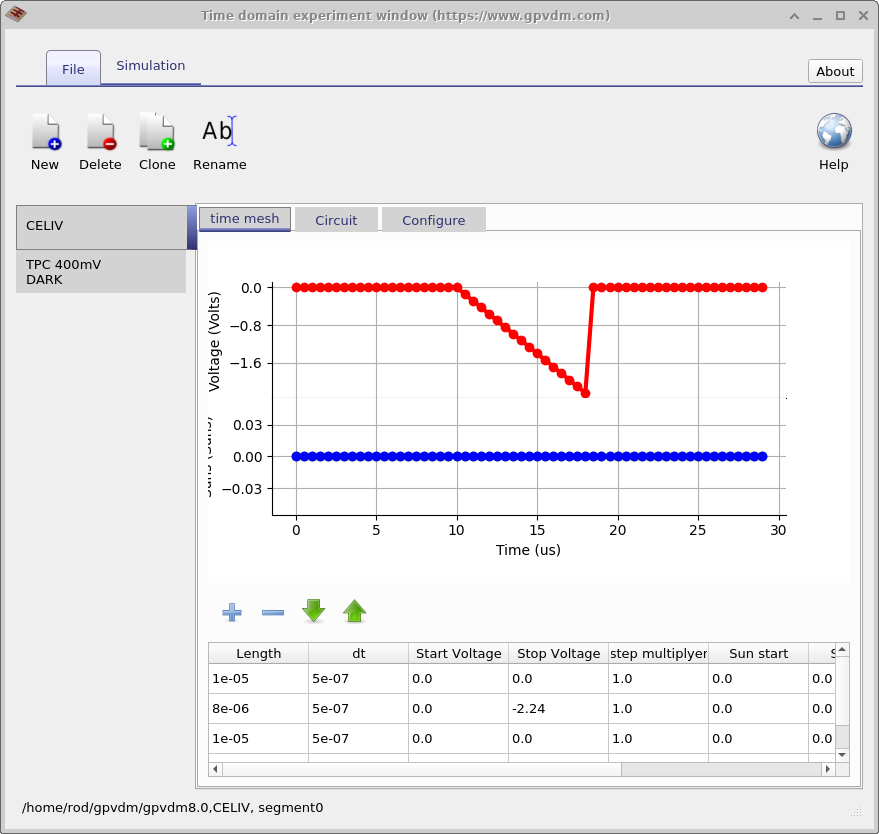
\includegraphics[width=0.5\textwidth,height=0.4\textwidth]{./images/time_domain_editor.png}

&
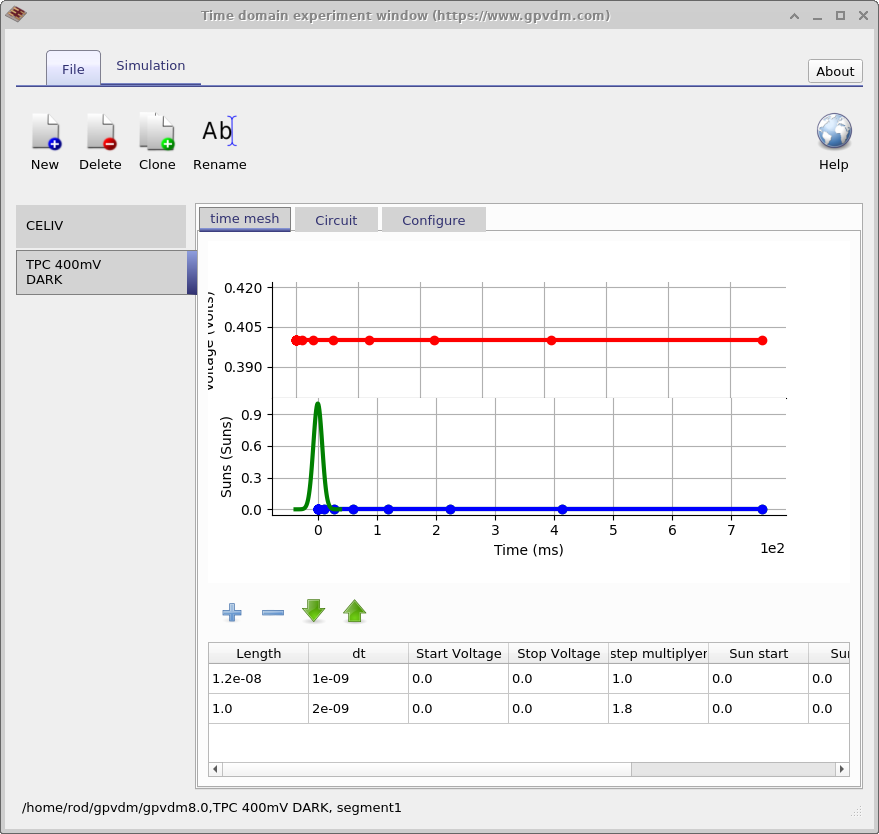
\includegraphics[width=0.5\textwidth,height=0.4\textwidth]{./images/time_domain_editor2.png}

\\

\end{tabular}
\caption{The time domain editor showing the user editing the duration of light/voltage pulses.}
\label{fig:timedomaineditor}
\end{figure}

Figure \ref{fig:timedomaineditor2} shows different tabs in of the time domain editor. The image on the left shows the circuit diagram used to model the CELIV experiment. From the left of the image the diode on the left accounts for the drift diffusion simulations it is in effect a perfect diode.  Then comes a capacitor used to model the charge on the plates of the device, then a shunt resistance and then the series resistance.  The final resistor on the right represents the external resistance of the measuring equipment.  The right hand figure shows the configuration options of the time domain window.

\begin{figure}[H]
\centering
\begin{tabular}{ c c }

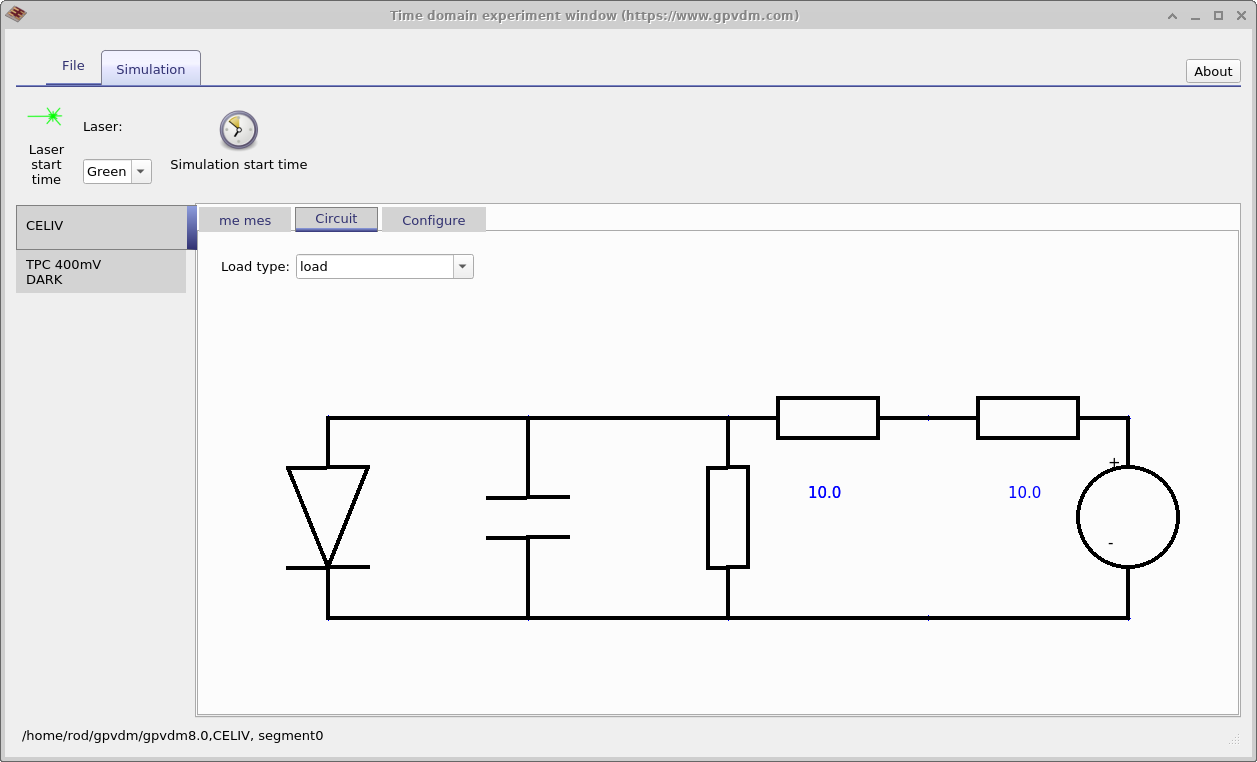
\includegraphics[width=0.5\textwidth,height=0.4\textwidth]{./images/time_domain_editor1.png}

&
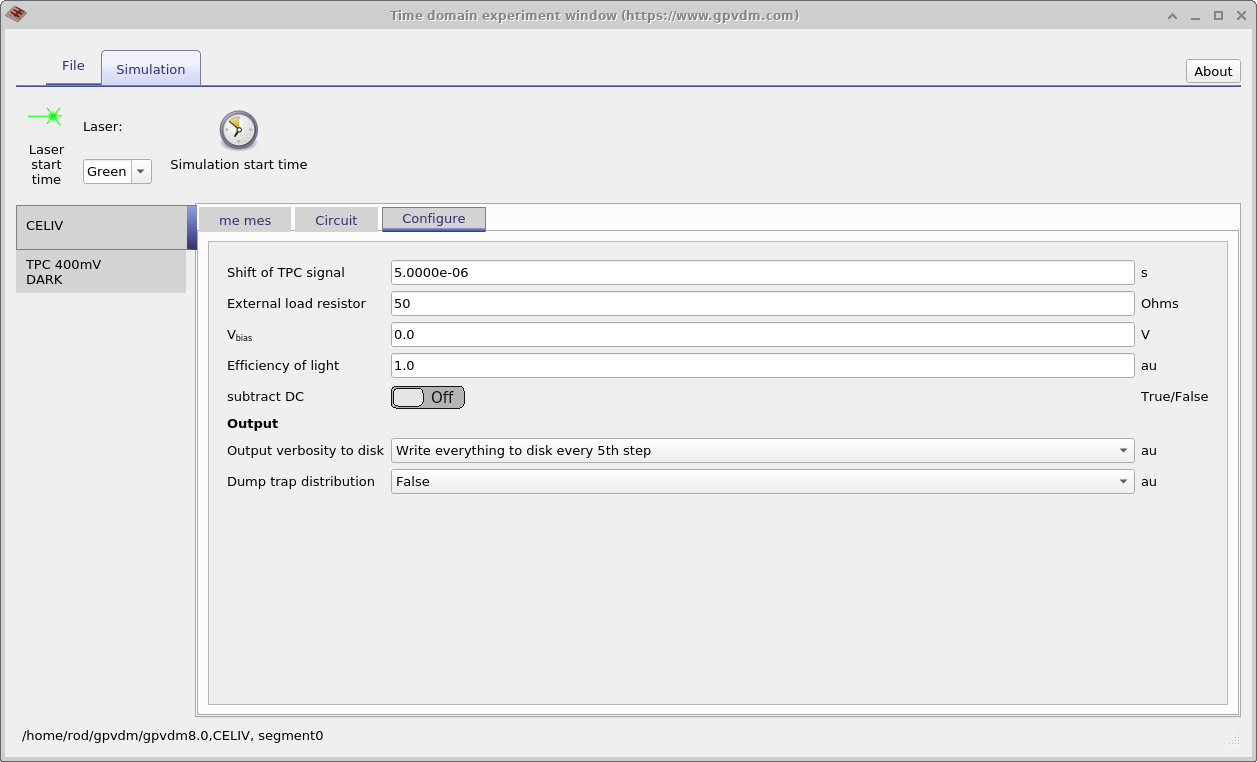
\includegraphics[width=0.5\textwidth,height=0.4\textwidth]{./images/time_domain_editor4.png}

\\

\end{tabular}
\caption{Configuring the time domain editor}
\label{fig:timedomaineditor2}
\end{figure}
